\documentclass[tikz,border=5mm]{standalone}
\begin{document}
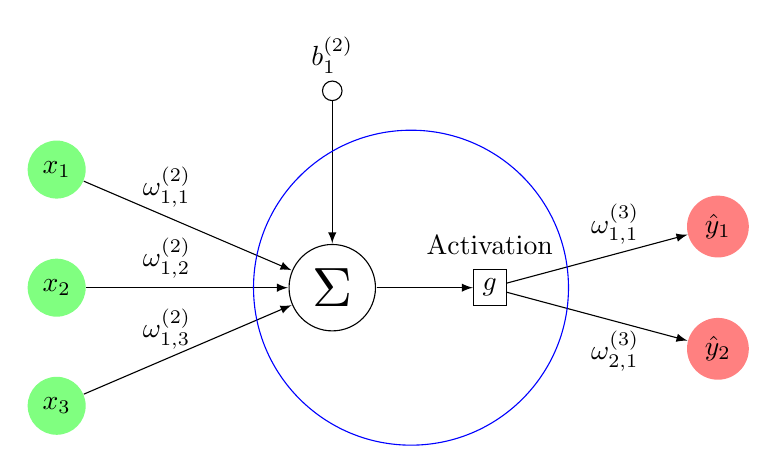
\begin{tikzpicture}[>=latex]
\path
(0,0)     node[circle,draw,scale=2,inner sep=2pt] (S) {$\Sigma$}
+(90:2.5) node[circle,draw,inner sep=2.5pt] (b) {}
          node[above=1mm] {$b_1^{(2)}$}
+(-3.5,1.5)  node[circle,fill=green!50]  (x1) {$x_1$}
+(-3.5,0)    node[circle,fill=green!50]  (x2) {$x_2$}
+(-3.5,-1.5) node[circle,fill=green!50]  (x3) {$x_3$}
(2,0)    node[draw] (g) {$g$} node[above=3mm]{Activation}
+(15:3)  node[circle,fill=red!50]  (y1) {$\hat{y}_1$}
+(-15:3) node[circle,fill=red!50]  (y2) {$\hat{y}_2$};
\draw[->] (S)--(g);
\draw[->] (b)--(S);
\draw[->] (g)--(y1) node[pos=.6,above]{$\omega_{1,1}^{(3)}$};
\draw[->] (g)--(y2) node[pos=.6,below]{$\omega_{2,1}^{(3)}$};
\draw[->] (x1)--(S) node[pos=.4,above]{$\omega_{1,1}^{(2)}$};
\draw[->] (x2)--(S) node[pos=.4,above]{$\omega_{1,2}^{(2)}$};
\draw[->] (x3)--(S) node[pos=.4,above]{$\omega_{1,3}^{(2)}$};
\draw[blue] (1,0) circle(2);
\end{tikzpicture}
\end{document}